\chapter{Reproducing the Results}
\label{app:repro}

All numbers, tables and figures in this report are produced by scripts from versioned data. On a laptop with Python~3.13:

\begin{verbatim}
python -m venv .venv && .venv/bin/pip install -e .[all] -r requirements.txt
# 1. dataset (needs free Alpaca keys; SEC EDGAR needs none)
.venv/bin/python scripts/build_dataset.py
# 2. main study: memory replay, both protocols, tables, figures 1-20
.venv/bin/python scripts/run_study.py --figures
# 3. LLM backbone experiment (needs free Groq keys)
.venv/bin/python scripts/run_llm_study.py
# 4. extension models: GRU, Transformer, Q-learning, analogues
.venv/bin/python scripts/run_extensions.py
# 5. figures 21-32 and LaTeX tables
.venv/bin/python scripts/make_extension_figures.py
.venv/bin/python scripts/export_latex_tables.py
.venv/bin/python scripts/export_extension_tables.py
.venv/bin/python scripts/crop_paper_screens.py   # screenshots sized for A4
# 6. tests and application
.venv/bin/python -m pytest -q
./run_dashboard.sh            # http://localhost:8050
\end{verbatim}

\chapter{Hyperparameters}
\label{app:hyper}

\begin{table}[H]
\centering
\small
\caption{Settings of every model. All were fixed before the test period was evaluated, except the two exploratory combinations.}
\label{tab:hyper}
\begin{tabular}{p{0.24\textwidth}p{0.68\textwidth}}
\toprule
Component & Settings \\
\midrule
FinMem & $Q=14/90/365$ days; $\alpha=0.9/0.967/0.988$; importance $v\in\{40,60,80\}$; purge at recency $<0.05$ or importance $<5$; access bonus $+5$; top-$K=5$ per layer \\
Ours (N1--N7) & FinMem core; hierarchical Beta--Bernoulli credibility (author $\rightarrow$ category $\rightarrow$ global, prior strength 8); duplicates: cosine $\ge0.88$ with the same polarity sign; contradiction: cosine $\ge0.72$, opposite polarity, $|s|\ge0.3$; 3 peers; episodic recall over the 10 nearest past contexts, at least 5 required \\
Threshold rule & $\theta\in\{0,0.05,0.1,0.15,0.2,0.3,0.4\}$, re-selected monthly on the previous 42 sessions \\
LightGBM & 200 trees, learning rate 0.03, 15 leaves, min.\ 40 samples per leaf, subsample 0.8, column sample 0.8, $\lambda=1$; 3 seeds \\
Logistic regression & standardised features, $C=0.5$ \\
GRU & 20-day window, 9 price features, hidden size 32, ticker embedding 4, dropout 0.2 \\
Transformer & 20-day window, $d=32$, 2 layers, 2 heads, feed-forward 64, dropout 0.1, learned positions, ticker embedding \\
Deep training & BCE loss, AdamW ($10^{-3}$, weight decay $10^{-3}$), batch 64, clip 1.0, $\le40$ epochs, early stopping patience 6 on the last 15\% of training rows, 3 seeds, monthly refit \\
Q-learning & 36 states, actions Flat/Long, $\alpha=0.1$, $\gamma=0.9$, 30 pre-training passes, $\varepsilon$ from 1 to 0.05, online updates in the test window, cost 5\,bps per switch \\
Pattern analogues & window 20 days, horizon 10 days, $k=8$, same-stock search, threshold 1\%, $P(\text{up})$ bounds 0.55/0.45 \\
Decision margin (ML/DL) & long if $P(\text{up})>0.52$, short if $<0.48$, otherwise keep \\
Costs & 5 basis points per unit of position change \\
Allocation back-test & 120-day estimation window, rebalance every 21 days, 20\% cash reserve, 25\% cap per stock \\
\bottomrule
\end{tabular}
\end{table}

\chapter{Application Programming Interface}
\label{app:api}

\begin{table}[H]
\centering
\small
\caption{Main HTTP endpoints of the application (JSON over HTTP on localhost).}
\label{tab:api}
\begin{tabular}{p{0.38\textwidth}p{0.55\textwidth}}
\toprule
Endpoint & Purpose \\
\midrule
\texttt{GET /api/portfolio} & account value, cash, positions, risk, orders \\
\texttt{GET /api/market\_data?ticker=} & daily OHLCV with indicators, live quote for today \\
\texttt{GET /api/agent/brief?ticker=} & retrieved memories, signals of the three memories, consensus \\
\texttt{POST /api/agent/llm} & LLM decision with the study prompt \\
\texttt{GET /api/agent/scan} & ten-stock scanner \\
\texttt{GET /api/research} & study results for the Research Lab \\
\texttt{GET /api/analytics/allocation} & budget split, rebalancing amounts, walk-forward comparison \\
\texttt{GET /api/analytics/analogs}, \texttt{/backtest}, \texttt{/sweep} & chart-pattern analogues and their evaluation \\
\texttt{GET /api/analytics/risk}, \texttt{/correlation}, \texttt{/portfolio} & risk report, correlation matrix, Monte Carlo equity distribution \\
\texttt{GET /api/analytics/algorithms}, \texttt{/experience}, \texttt{/rl} & algorithm board, decision log, Q-learning agent \\
\texttt{GET /api/autopilot/status} & limits, configuration, approval queue, activity log \\
\texttt{POST /api/autopilot/config} & save budget, limits and autopilot settings \\
\texttt{POST /api/autopilot/run\_once}, \texttt{/resolve}, \texttt{/kill}, \texttt{/resume}, \texttt{/rebalance} & run a check, approve/reject, emergency stop, resume, queue a rebalance \\
\texttt{GET /api/credentials}, \texttt{POST /api/credentials/save|test|remove} & key status (masked), verify and store, test, remove \\
\bottomrule
\end{tabular}
\end{table}

\chapter{User Guide (English and Bangla)}
\label{app:guide}

\begin{enumerate}
  \item \textbf{Connect accounts} (Settings $\rightarrow$ Connections): paste the Alpaca \emph{paper} key and secret and at least one Groq or OpenRouter key, then press \emph{Save \& test}. Only keys that the provider accepts are saved.
  \item \textbf{Set the budget} (Settings $\rightarrow$ Budget \& limits): total budget, cash to keep, the most that may go into one stock or one order, the daily-loss and drawdown limits and the stocks the AI may buy. A sentence under the form explains the limits in plain words.
  \item \textbf{Choose a stock} with the picker at the top; every page follows it.
  \item \textbf{Look before acting}: the Home page shows the AI's view in plain words, the Trade page the chart signals, the Insights pages the budget split, similar past charts, possible futures, risk, correlation and what every algorithm says with its track record.
  \item \textbf{Let the AI work}: on the AI Autopilot page choose how much freedom it gets (start with \emph{Ask me first}), how it decides and how often it checks, then start it. Approve or reject its proposals in the queue; the emergency stop halts everything.
  \item \textbf{Language and theme}: switch between English and Bangla and between light and dark mode in the top bar.
\end{enumerate}

\begin{figure}[H]
\centering
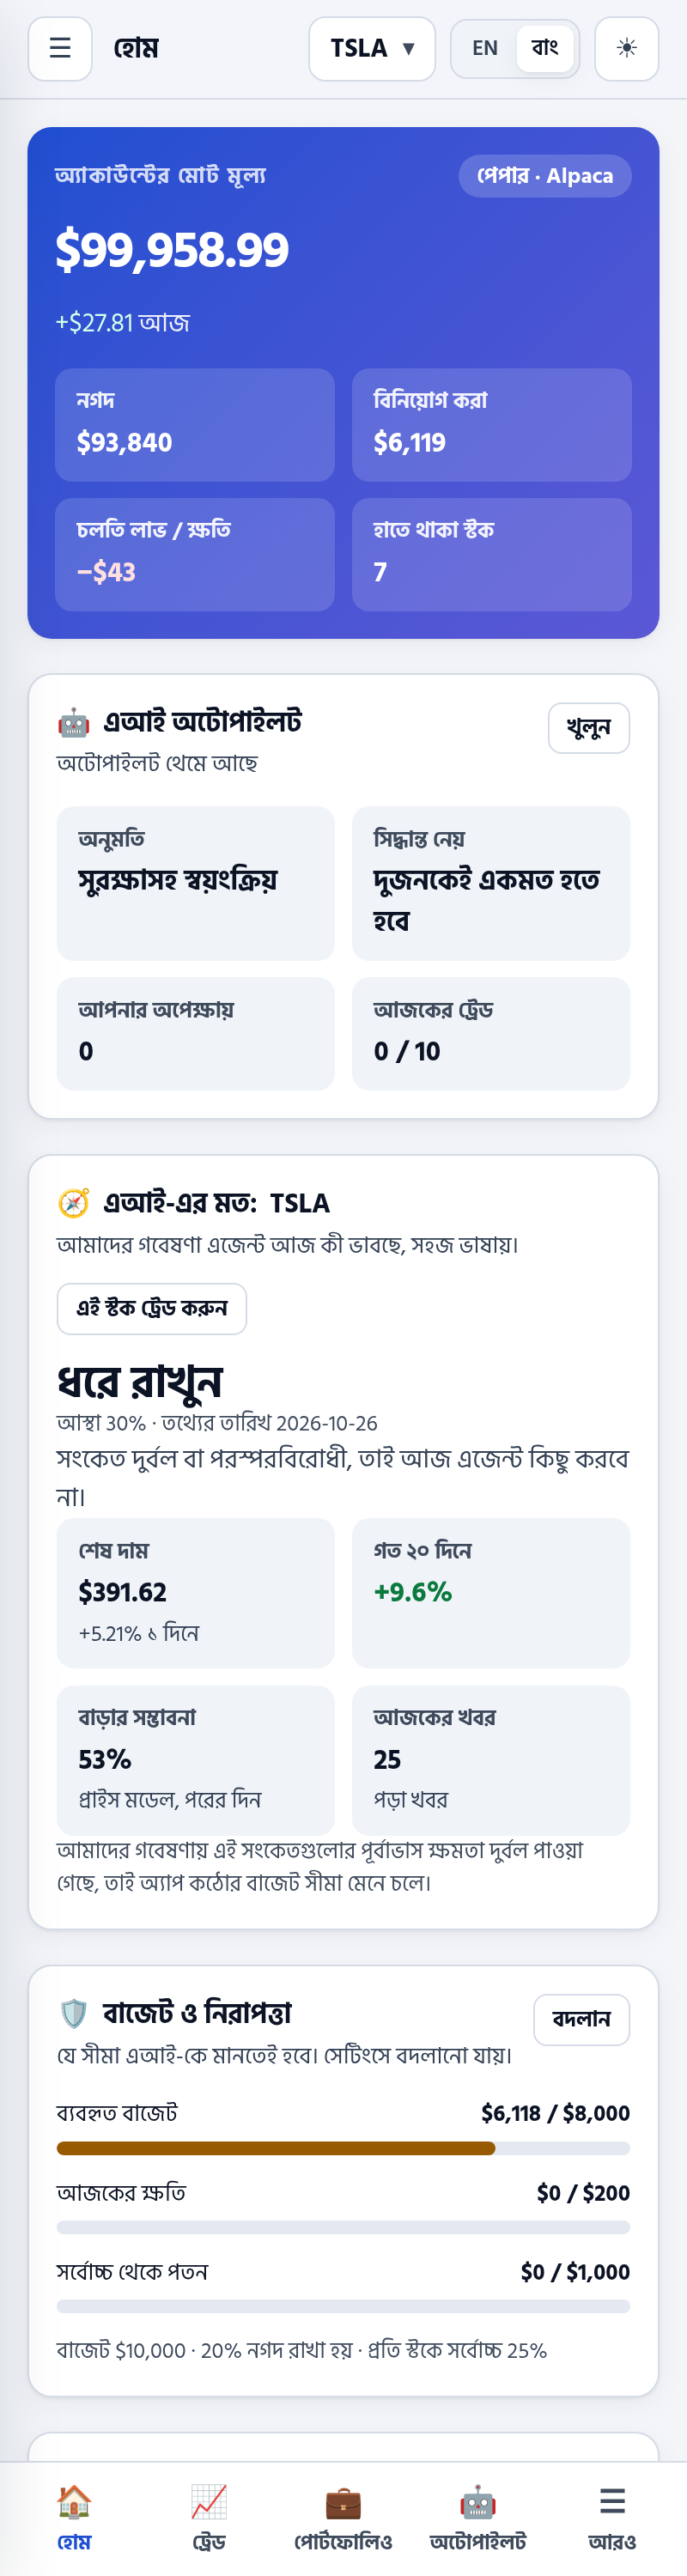
\includegraphics[height=0.8\textheight]{app_mobile_home_bn.png}
\hspace{0.03\textwidth}
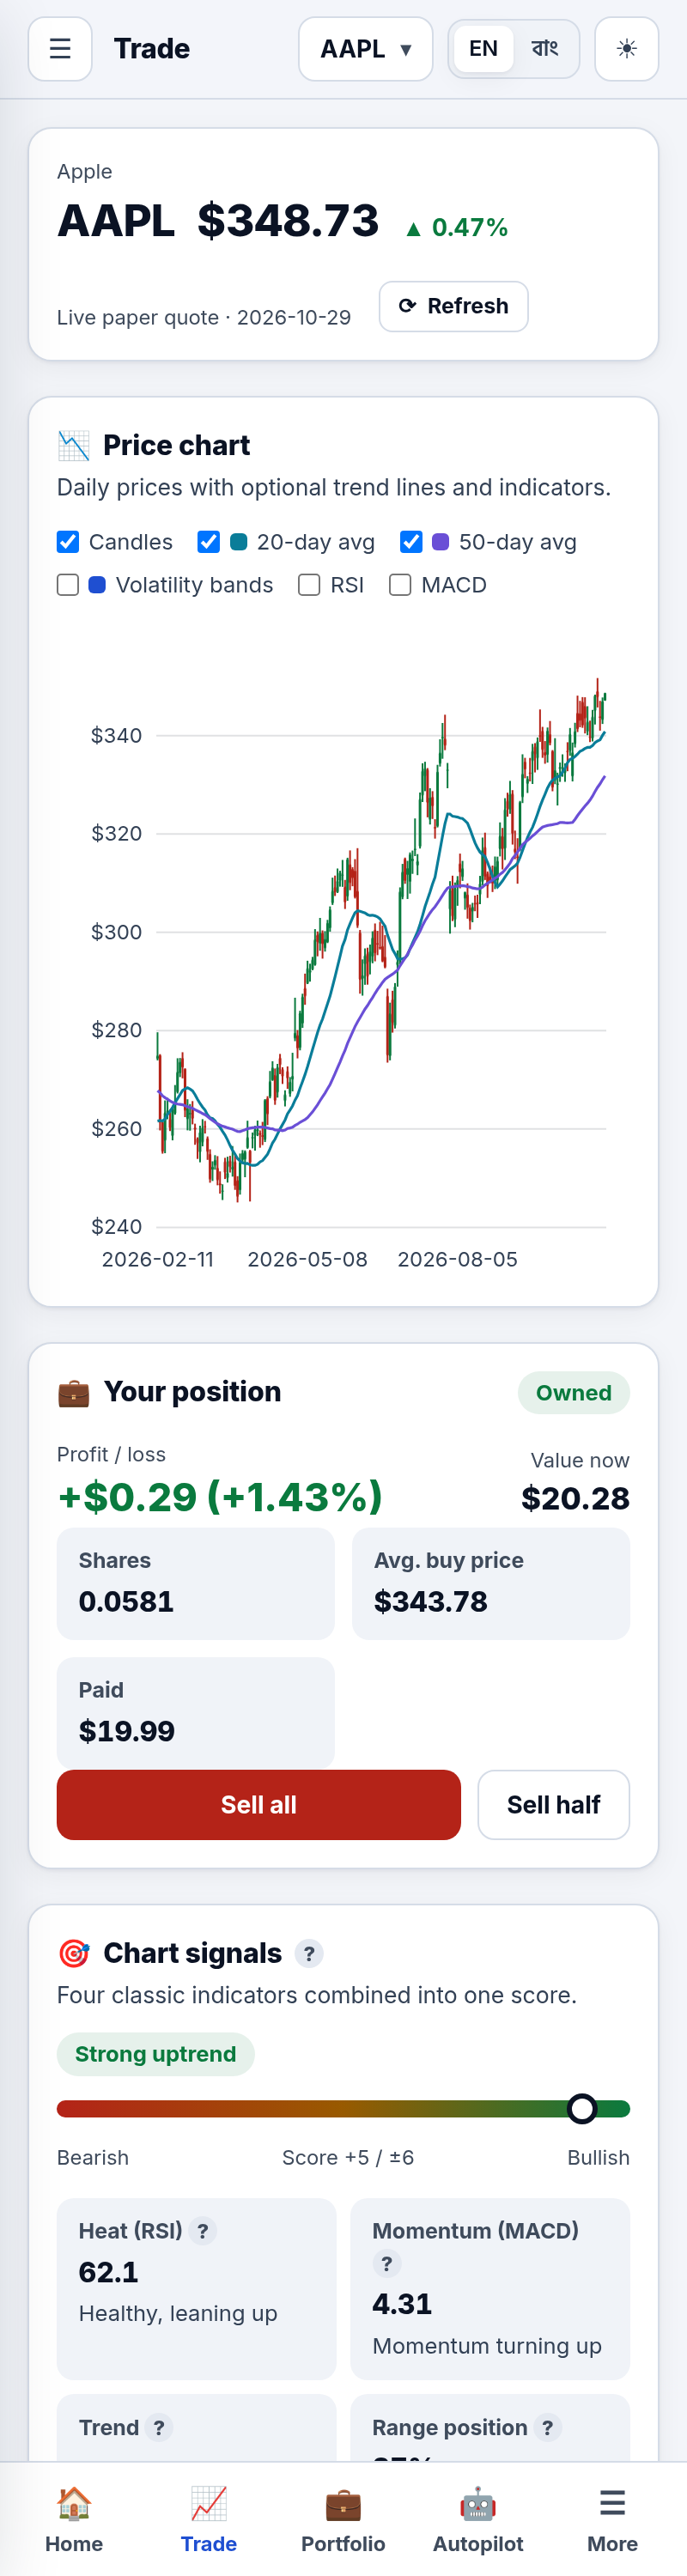
\includegraphics[height=0.8\textheight]{app_mobile_trade.png}
\caption{The application on a phone: Home in Bangla (left) and Trade in English (right).}
\label{fig:ui-mobile}
\end{figure}
